\documentclass[12pt,letterpaper]{article}
\usepackage{amsmath,amsthm,amsfonts,amssymb,amscd}
\usepackage{listings}
\usepackage{color}

\definecolor{dkgreen}{rgb}{0,0.6,0}
\definecolor{gray}{rgb}{0.5,0.5,0.5}
\definecolor{mauve}{rgb}{0.58,0,0.82}

\lstset{%frame=tb,
  language=Bash,
  aboveskip=3mm,
  belowskip=3mm,
  showstringspaces=false,
  columns=flexible,
  basicstyle={\small\ttfamily},
  numbers=none,
  numberstyle=\tiny\color{gray},
  %keywordstyle=\color{blue},
  %commentstyle=\color{dkgreen},
  stringstyle=\color{mauve},
  breaklines=true,
  breakatwhitespace=true
  tabsize=3
}


\usepackage{hyperref}
\usepackage{graphicx}
\usepackage{enumerate}
\usepackage{fancyhdr}
\usepackage{mathrsfs}
\usepackage[margin=3cm]{geometry}
\setlength{\parindent}{0.0in}
\setlength{\parskip}{0.05in}

% Edit these as appropriate
\newcommand\course{CS595}
\newcommand\semester{FAll 2013}     
\newcommand\hwnum{4}
\newcommand\yourname{Mohamed Aturban}
\newcommand\login{maturban}

\newenvironment{answer}[1]{
  \subsubsection*{Problem #1}
}

\pagestyle{fancyplain}
\headheight 40pt
\lhead{\yourname\ (\login)\\\course\ --- \semester}
\chead{\textbf{\Large Assignment \hwnum}}
\rhead{\today}
\headsep 40pt

\begin{document}

All files mentioned in this document should be uploaded into the {\it github} repository.

\begin{answer}{1}
The Python program {\it q1.py} is the answer to question 1. The code will do the following. It starts by choosing the first 100 active links stored in the file {\it links.txt}. For each URI, all {\bf distinct} outbound links from that page are extracted then stored in a separate file. For Example, \url{http://avimeo.com/watch.php?vid=12dd9a60d#.UkGBQQq-0Nk.twitter} is the fifth active link in {\it links.txt}, so the program will create a file called {\it f5.txt} which looks like:

\begin{lstlisting}
	# The first link is the main page in which other
	# URIs ,starting from second link , are extracted.
	http://avimeo.com/watch.php?vid=12dd9a60d#.UkGBQQq-0Nk.twitter
	http://avimeo.com/index.php
	http://avimeo.com/login.php
	http://avimeo.com/register.php
	...
	
\end{lstlisting}

As you can see, the first two lines are just comments describing the contents of the file. The first URI is the main page from which other links are extracted, starting from second link.

\end{answer}


\begin{answer}{2}

The main task of  {\it q2.py}  is to create a {\it GraphViz dot} file called {\it graphLinks.gv} which can be used as input to {\it Gephi}. The following four points briefly illustrate how the dot file is created:

\begin{itemize}
\item Read one file (e.g. f1.txt) of 100 files
\item Extract the main URI ({\it m}) and the outbound links ({\it l1,l2,l3, ...})
\item Before labeling edges between {\it m} and outbound links {\it l}, check if these nodes are already given labels. In this case, they will not be offered new labels. Instead. they will keep their old labels.
\item Create and label node pairs :  {\it m} $\rightarrow$ {\it l} [label = "{\it m}\# to {\it l}\#" ]
\item Assign labels to new nodes: 

	{\it m} [label = {\it m}\# ]	or
	
	{\it l} [label = {\it l}\# ]

\item Repeat previous five steps for all 100 files.

\end{itemize}

Again, the output dot file is called {\it graphLinks.gv}.

\end{answer}

\begin{answer}{3}

After Loading the dot file {\it graphLinks.gv} created in problem 2 into Gephi, we get the following graph (figure 1). It is difficult to organize the graph in a certain way that shows its connectivity since there are thousands of edges.

\begin{figure}[ht!]
\centering
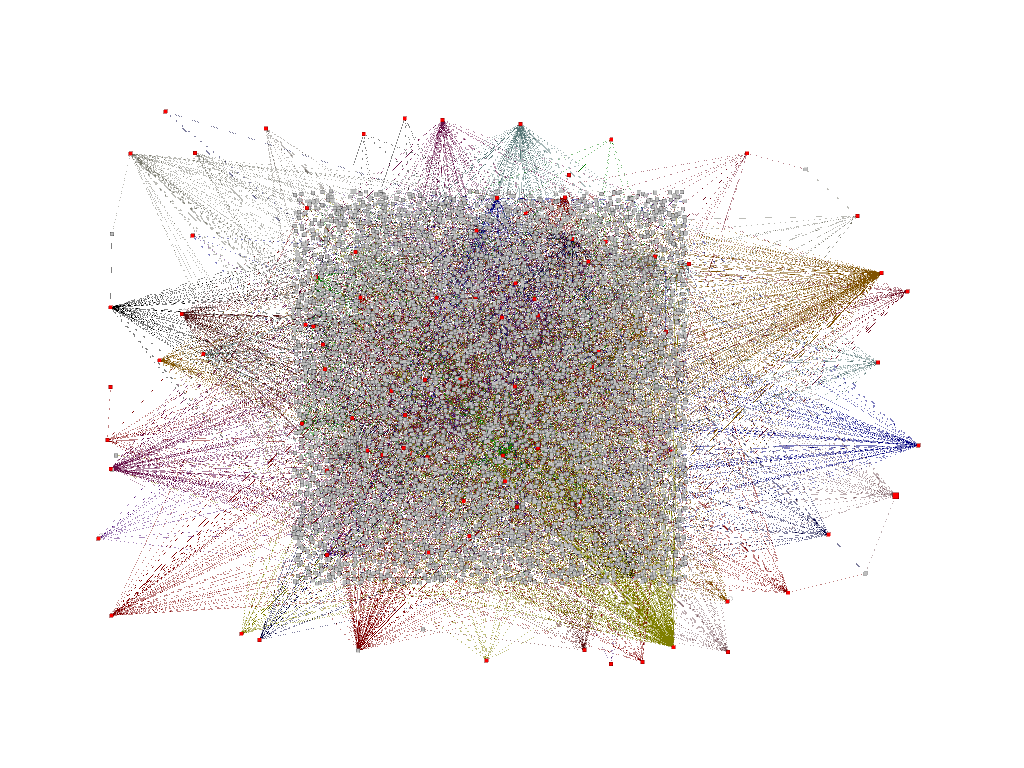
\includegraphics[scale=0.55]{all}
\caption{Graph with all nodes}
\label{overflow}
\end{figure}

Figure 2 shows examples of connected components such as:

\begin{itemize}
\item Node no. 10.4 is connected to main nodes: 10, 75, and 76
\item Node no. 9.45 is connected to main nodes: 9 and 12
\item Node no. 81.17 is connected to main nodes: 81 and 83

...

\begin{figure}[ht!]
\centering
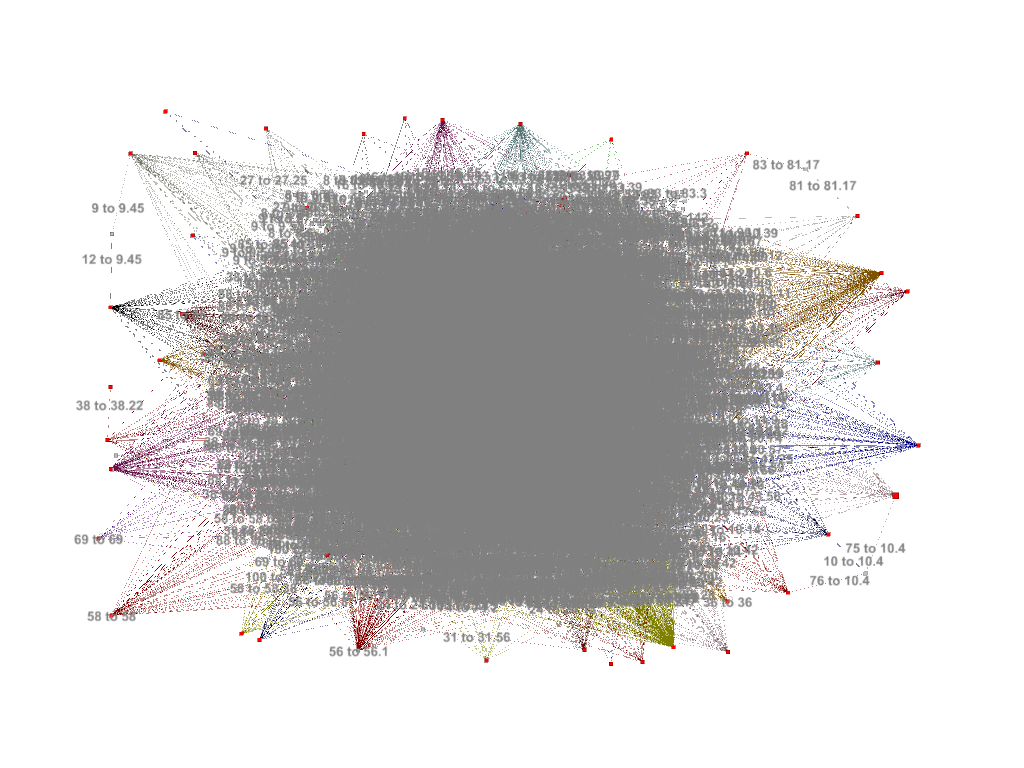
\includegraphics[scale=0.55]{lablel}
\caption{Graph : Connected nodes}
\label{overflow}
\end{figure}


Other statistics:
\item Average Degree: 1.089

\begin{figure}[ht!]
\centering
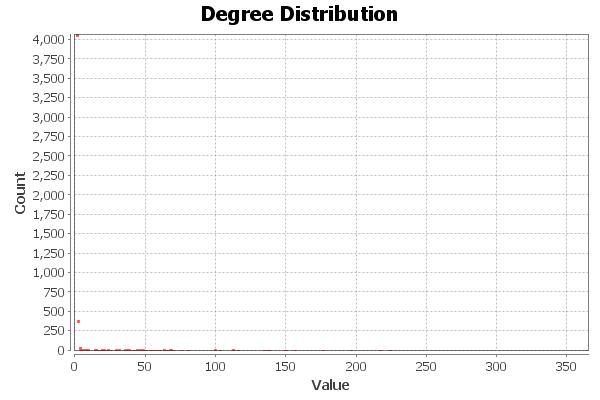
\includegraphics[scale=0.55]{degree-distribution}
\caption{degree-distribution}
\label{overflow}
\end{figure}

\begin{figure}[ht!]
\centering
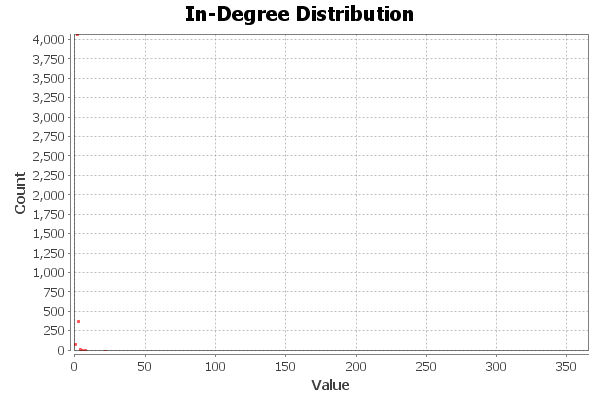
\includegraphics[scale=0.55]{indegree-distribution}
\caption{indegree-distribution}
\label{overflow}
\end{figure}

\begin{figure}[ht!]
\centering
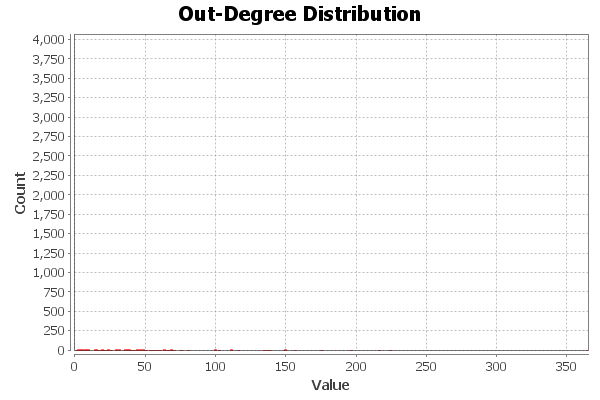
\includegraphics[scale=0.55]{outdegree-distribution}
\caption{outdegree-distribution}
\label{overflow}
\end{figure}

\item Number of Weakly Connected Components: 58
\item Number of Stronlgy Connected Components: 4577


\begin{figure}[ht!]
\centering
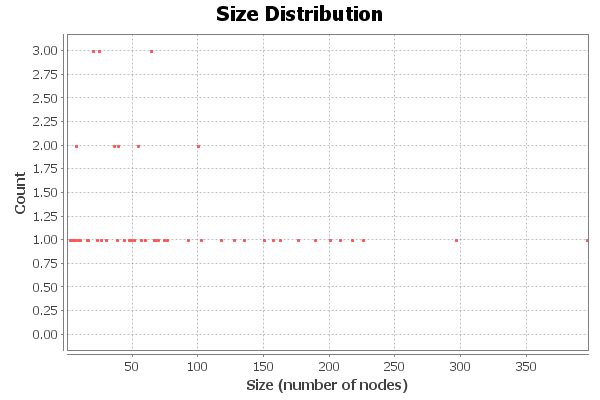
\includegraphics[scale=0.55]{cc-size-distribution}
\caption{cc-size-distribution}
\label{overflow}
\end{figure}


\begin{figure}[ht!]
\centering
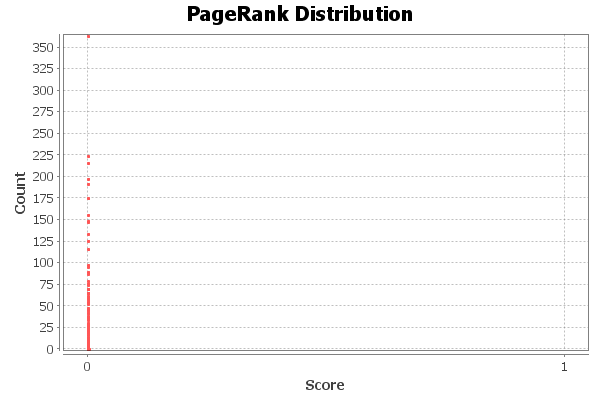
\includegraphics[scale=0.55]{pageranks}
\caption{pageranks}
\label{overflow}
\end{figure}


\begin{figure}[ht!]
\centering
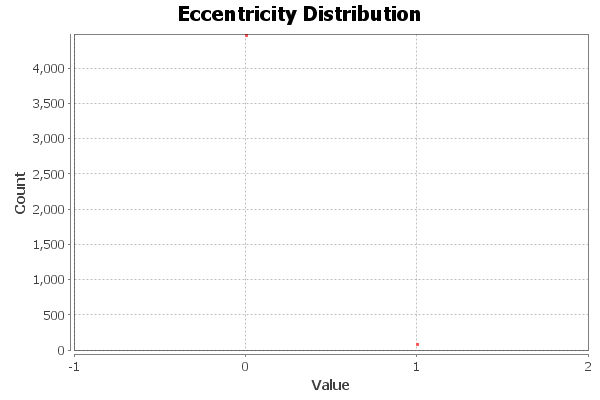
\includegraphics[scale=0.55]{EccentricityDistribution}
\caption{Eccentricity Distribution}
\label{overflow}
\end{figure}

\begin{figure}[ht!]
\centering
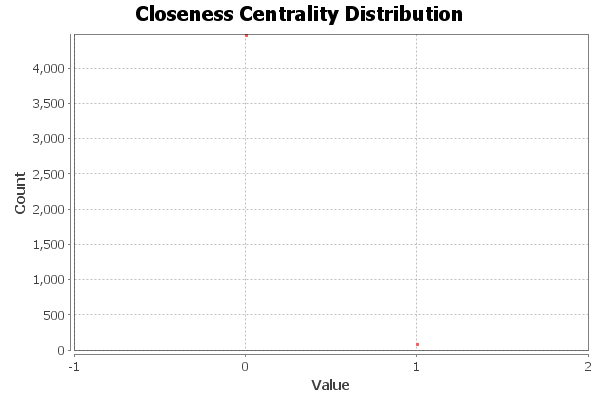
\includegraphics[scale=0.55]{ClosenessCentralityDistribution}
\caption{Closeness Centrality Distribution}
\label{overflow}
\end{figure}

\begin{figure}[ht!]
\centering
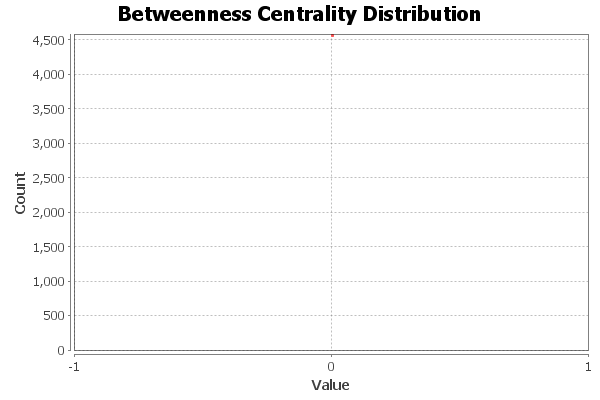
\includegraphics[scale=0.55]{BetweennessCentralityDistribution}
\caption{Betweenness Centrality Distribution}
\label{overflow}
\end{figure}

for more details, there is more statistical detail uploaded into the repository.

\end{itemize}




\end{answer}


\end{document}
